\documentclass[11pt]{sdm}
\usepackage{xcolor}
\usepackage{float}
\usepackage[utf8]{inputenc} 
\usepackage{indentfirst}
\usepackage{listings}
\usepackage{hyphsubst}
\usepackage{amsmath}

				  
\lstdefinestyle{customc}{
  belowcaptionskip=1\baselineskip,
  breaklines=true,
  frame=L,
  xleftmargin=\parindent,
  language=C,
  showstringspaces=false,
  keywordstyle=\bfseries\color{green!40!black},
  commentstyle=\itshape\color{purple!40!black},
  identifierstyle=\color{blue},
  stringstyle=\color{orange},
}

\lstset{escapechar=@,style=customc}


%Number the pages
\pagestyle{plain}

\title{Software Fault Isolation using the CompCert compiler}
\author{Alexandre \textsc{DANG}}
\supervisorOne{Frédéric \textsc{Besson}}
\team{Team CELTIQUE}

\school{supelec}

\domain{Domaine: Cryptography and Security}

%write your abstract here
\abstract{}

\begin{document}
\maketitle

%*****************************************************************%

\section{Introduction}


\begin{itemize}
	\item Secure malicious code through software solution
	\item Usage in applications which use modules from unknown origin (browsers, computer clusters)
	\item current appeal for SFI speed and small TCB
	\item SFI is still incomplete, especially with ROP attack => our approach
	\item  plan
\end{itemize}


\section{\textit{Software Fault Isolation}}
	We introduce here \textit{Software Fault Isolation} (SFI) which inspired us the idea to protect return addresses through fixed stack frame size. SFI aims to protect a main program from the different modules that he will need to use. These modules will be loaded in the same memory space as the main program but in a confined area called \textit{sandbox}. The SFI mechanism is composed of two elements: a code generator and a verifier. The generator transforms the assembly code of the hazardous modules so that they will be constrained in the sandbox. The verifier operates just before loading the modules in the memory. It checks the if SFI transformations introduced by the generator are still present and valid. For the rest of the document we will reserve the word ''program'' to refer to the code protected by SFI and ''module'' to refer to the hazardous code.

\subsection{Principle}

The main principle behind SFI was first presented in the work of Wahbe and al. \textcolor{green}{ref}
. Later works \textcolor{green}{ref}, which will be introduced in the chapter \ref{ssub:Implementations}, are all based on the foundations of SFI detailed here.
The implementation described here was realised for a RISC architecture like MIPS or \textit{Alpha}.

SFI considers that a malicious code is effectively contained in the sandbox if these three security properties hold true:
\begin{itemize}
	\item \textbf{Verified code}, only instructions that have been checked by the verifier will be executed 
	\item \textbf{Memory safety}, malicious modules won't do any \textit{write} or \textit{jump} operations out of the sandbox
	\item \textbf{Flow control integrity}, every flow control transfer from hazardous modules to the main program is identified and verified
\end{itemize}
The first property protects us against self-modifying code which could bypass the SFI measures. \textit{Memory safety} prevents any illegal access to the memory of the protected program. The last property allows us to authorized only licit interactions between the program and its modules. SFI forbids any call from malicious modules that could modify the flow control of the program. If the flow control was fiddled with, it could lead to an unexpected behaviour of the program which we want to avoid.

The code generator transforms the assembly code of the hazardous modules so that respect the security properties presented before. The generator is integrated to the compiler which will create \textit{sandboxed executable}. Afterwards this executable will be checked by the verifier before being loaded in the memory. 
It verifies that the transformations introduced by the generator are present and valid. If the verification fails the module will be rejected and won't be executes. We can note that we only need to trust the verifier to prevent running any dangerous module. It's one advantage of SFI, only the verifier needs to be in the \textit{Trusted Computing base} (TCB).


\subsubsection{Code generator}
\label{ssub:Code generator}
To protect the program from its modules, the generator will restrain every write and jump instructions of the modules to addresses of their sandbox.
The generator has to face three issues to do so. Firstly, is to introduce protection mechanisms before every dangerous instructions. For example, assessing that the address of a jump instruction is an authorized one.
Secondly, we have to make sure that these protection mechanisms can't be avoided. 
Finally, the transformations introduced have to authorized only legal calls out of the sandbox by using entry points specified by the protected program. For example, Google Chrome only allows its modules to use a specific interface to interact with the browser. This way the modules can't disrupt the flow control of Google Chrome easily.
\paragraph{Confining memory accesses}
\label{par:Confining memory accesses}
The main program memory should avoid being corrupted by its modules. SFI aims to isolates these modules in a reserved of the program's memory called sandbox.
The sandbox is a contiguous memory area which size is a power of two. Indeed, these requirements eases the confinement of the modules in their sandbox by using arithmetic operations on bits which accelerates the process.
\paragraph{Protection of sandboxing mechanisms}
\label{par:Protection of sandboxing mechanisms}
\paragraph{Controlled interactions with the protected program}
\label{par:Controled interactions with the protected program}

\subsubsection{Code verifier}
\label{ssub:Code verifier}

\subsubsection{Pros and cons}
\label{ssub:Pros and cons}

\subsubsection{Implementations}
\label{ssub:Implementations}
\paragraph{NativeClient, SFI for Google Chrome}
\label{par:NativeClient, SFI for Google Chrome}


\subsection{SFI using CompCert}

\subsubsection{CompCert the verified compiler}
\label{ssub:CompCert the verified compiler}
\paragraph{CompCert}
\label{par:CompCert}
\paragraph{Memory model of CompCert}
\label{par:Memory model of CompCert}


\subsubsection{SFI with CompCert}
\label{ssub:SFI with CompCert}
\paragraph{Cminor}
\label{par:Cminor}
\paragraph{Specification of the SFI transformation}
\label{par:Specification of the SFI tranformation}
\paragraph{Masking in CompCert}
\label{par:Masking in CompCert}




\subsubsection{Evalutation of the approach}
\label{ssub:Evalutation of the approach}

\subsection{Limits of SFI}
\label{sub:Limits of SFI}
\subsubsection{Return addresses}
\label{ssub:Return addresses}
\subsubsection{Proposed solution}
\label{ssub:Proposed solution}


\section{Protecting the stack with fixed frame size}
\label{sec:Protecting the stack with fixed frame size}
	A lot of attacks on software aims to interfere with the control flow of the targeted program. Among those, \textit{Returned Oriented Programming} (ROP) attacks specifically try to overwrite the return addresses.
By doing so the attacked function will return to a malicious piece of code that will get executed (see Figure \ref{rop_attack}).
Stack overflow is an example of such ROP attacks.
We propose a solution against ROP attacks which combined with SFI would protect from most of control-flow interference attacks.
Inspired from SFI techniques we aim to prevent any overwriting of the return addresses. To do so we need to know these return addresses location in the memory. Therefore our approach consists of modifying the stack structure in order to have an easy way to know the return addresses locations. With this knowledge we will be able to put a mask, as in SFI, before every dangerous write instructions and prevent any ROP attack.

\begin{figure}
\centering
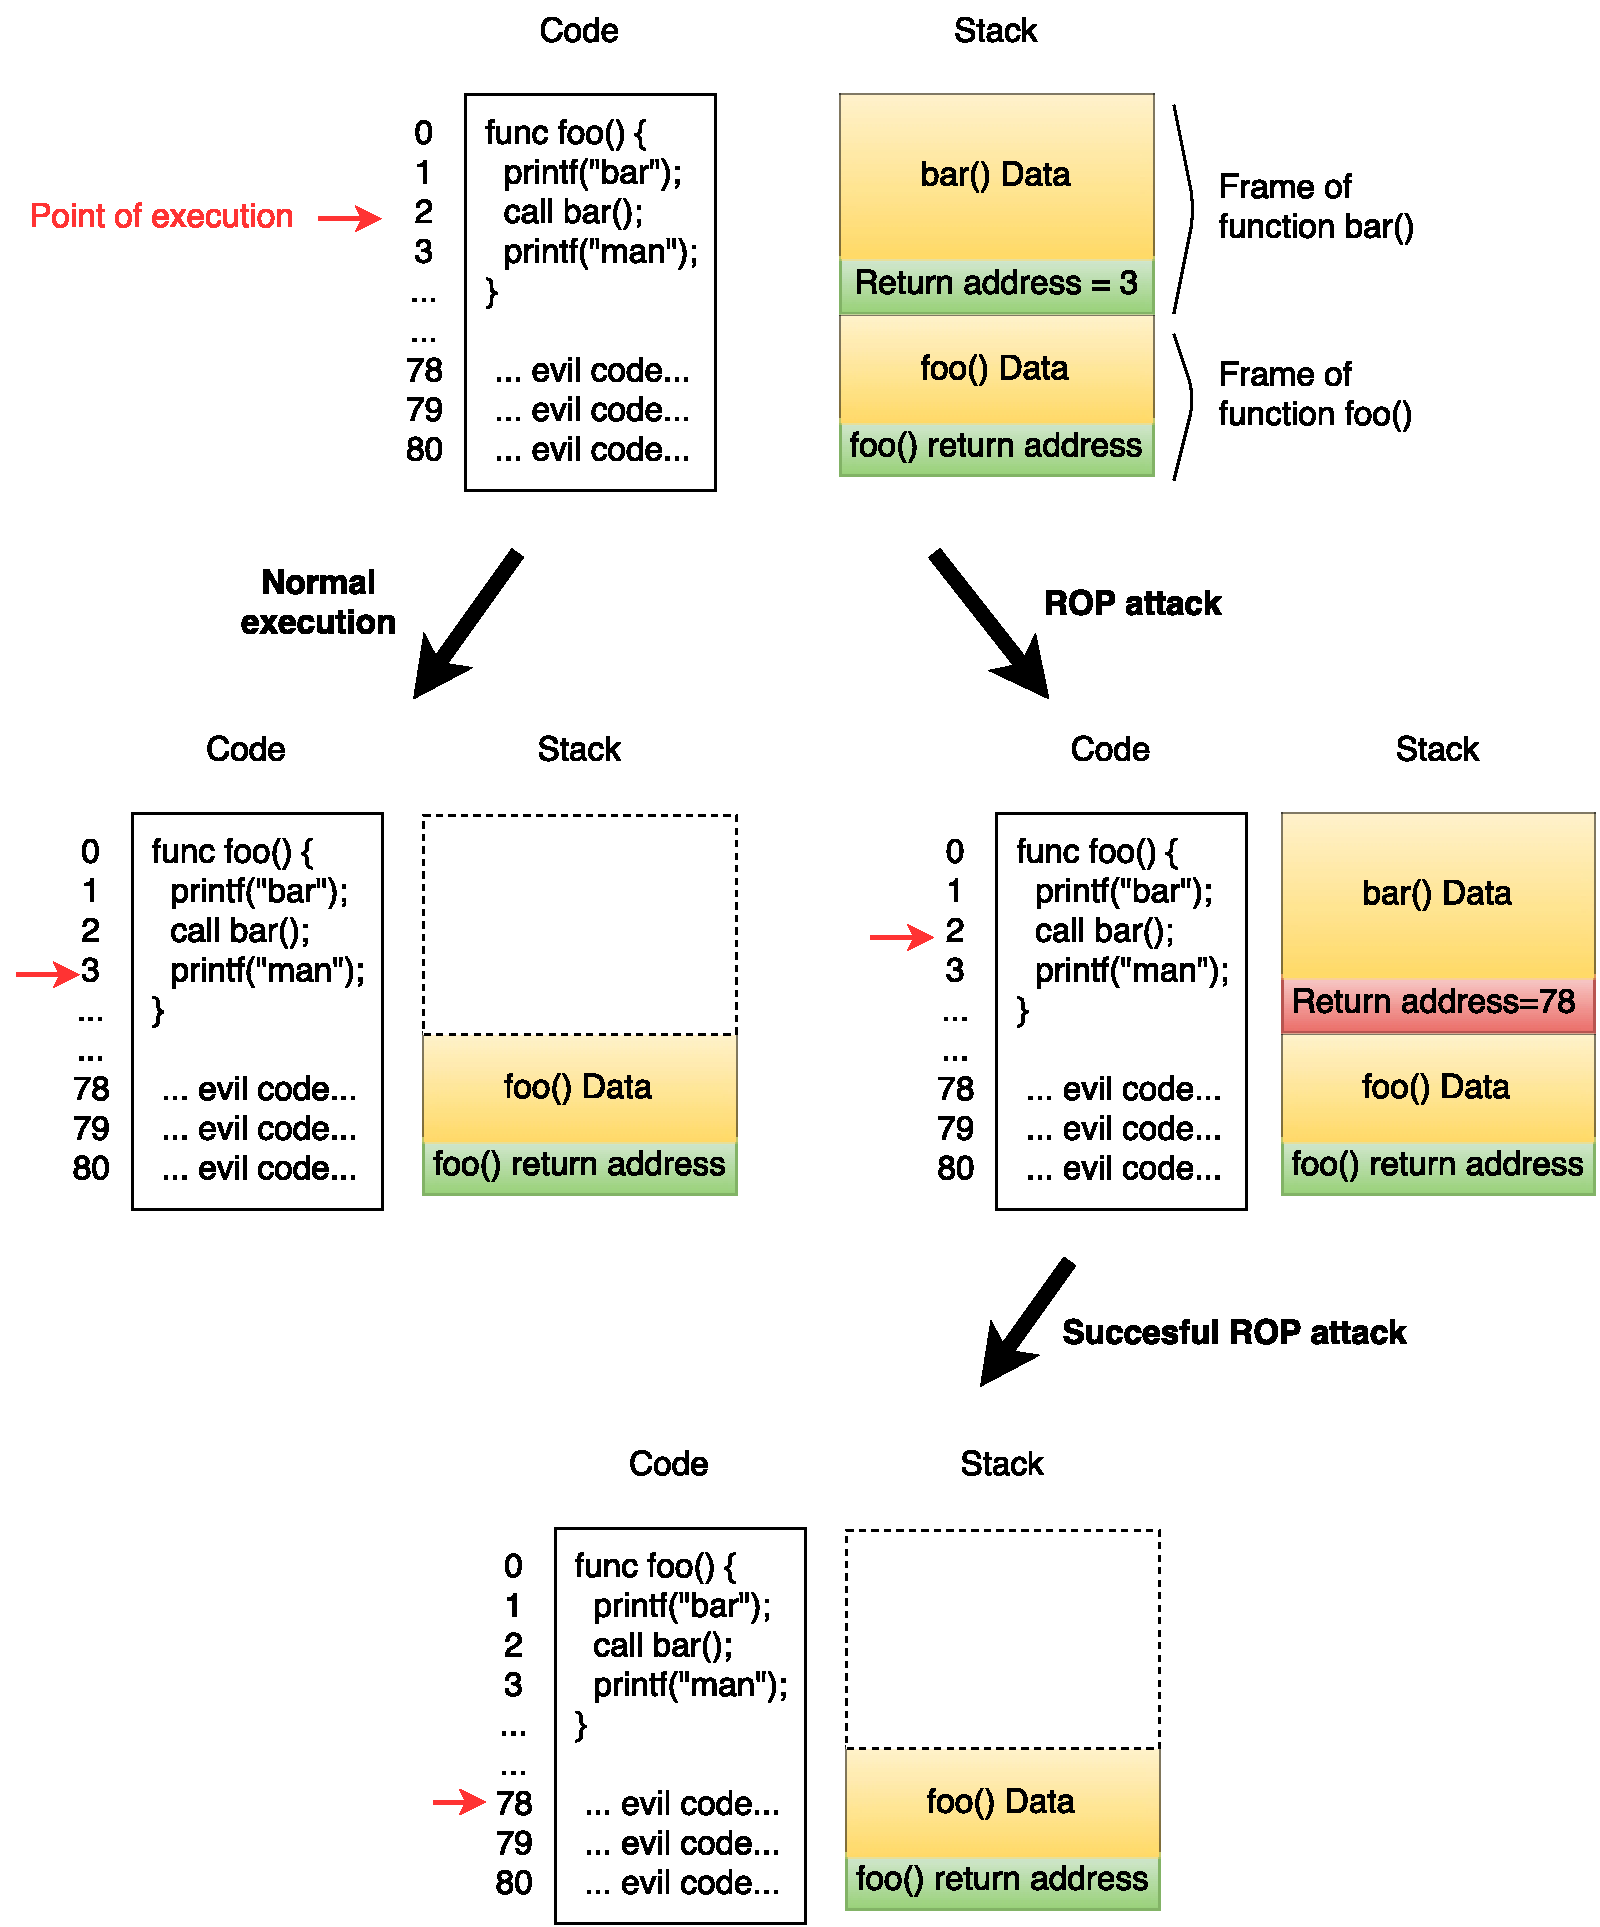
\includegraphics[scale=0.6]{images/rop_attack.pdf}
\caption{ROP attack}
\label{rop_attack}
\end{figure}

\subsection{Description of the approach}
\label{sub:Description of the approach}

\subsubsection{Issue}
\label{ssub:Issue}

	We want to protect the return addresses in the stack from being overwritten illegally. The only moment they should be written over is during a function call routine.
We want to use a masking operation similar as in SFI, therefore we need to be able to check if an address is the location of a return address. One solution to enable these runtime checks is to enforce a strict control over the stack, thus allowing us to know the exact locations of the return addresses.
\textcolor{green}{suggest another idea maybe}

\subsubsection{Proposed solution}
\label{ssub:Proposed solution}

	To be able to know the return addresses location we suggest a solution.
The idea is to define a constant size for the frames of the stack. Stack frames are created and added to the stack after every function call, whereas they are removed from the stack when returning from the calling function. The frames are piled up on the stack following the FIFO rule (\textit{First In First Out}).
In these frames the return addresses usually have a specific place, and by fixing the frames size we impose the return addresses to have a fixed offset between them.
With this property we can guess the location of every return address which would be: $ \mathbf{c~mod~n} \text{     with } c \text{ a constant and } n \text{ the size of the frames }$.
Now that we know $n$ (the size of the frames), we need to get the constant $c$. To solve this, our idea is to align the beginning of the stack when starting the program. This way we can choose the constant $c$ and we arrange it to have $c=0$.
More details can be seen on Figure \ref{stack_transform}.

\begin{figure}
\centering
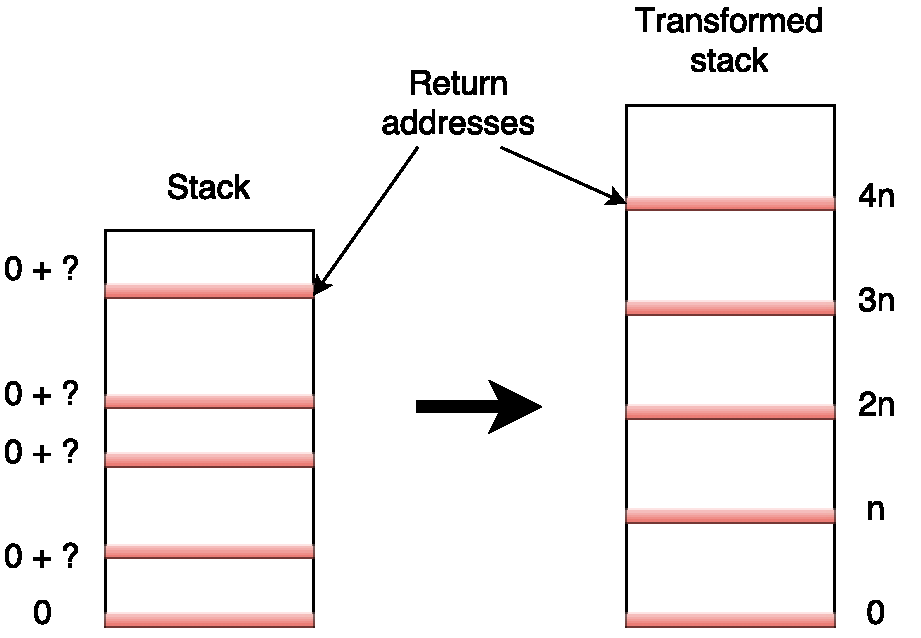
\includegraphics[scale=0.5]{images/stack_transform.pdf}
\caption{Stack modifications}
\label{stack_transform}
\end{figure}

The second step is to detect every possibly harmful to return addresses (Figure \ref{dangerous_statement}). All the operations which can write in the memory can be considered dangerous. Hence we target all instruction related to variable assignment. If we want more precision, we can also target assignments to variables located on the stack.

\begin{figure}
\begin{lstlisting}
int foo(int a) {
	int* pointer = &a;
	//In pointer we get the address of the parameter a which is in the stack

	*(pointer+4) = 0xff000000;
	//We write the value 0xff000000 in the stack
	//if this location is a return address, the ROP attack succeeds
}
\end{lstlisting}
\centering
\caption{Example of dangerous C statement}
\label{dangerous_statement}
\end{figure}

Finally when we have detected all the dangerous statements we transform the module code. Before each of this dangerous statement we add a protection mechanism similar to masking in SFI. If the address written does not match the location of a return address, then the operation is allowed and the program continues to run casually. Whereas if there is an attempt to write on a return address we trigger an error behaviour like crashing (Figure \ref{runtime_check}).

\begin{figure}
\centering
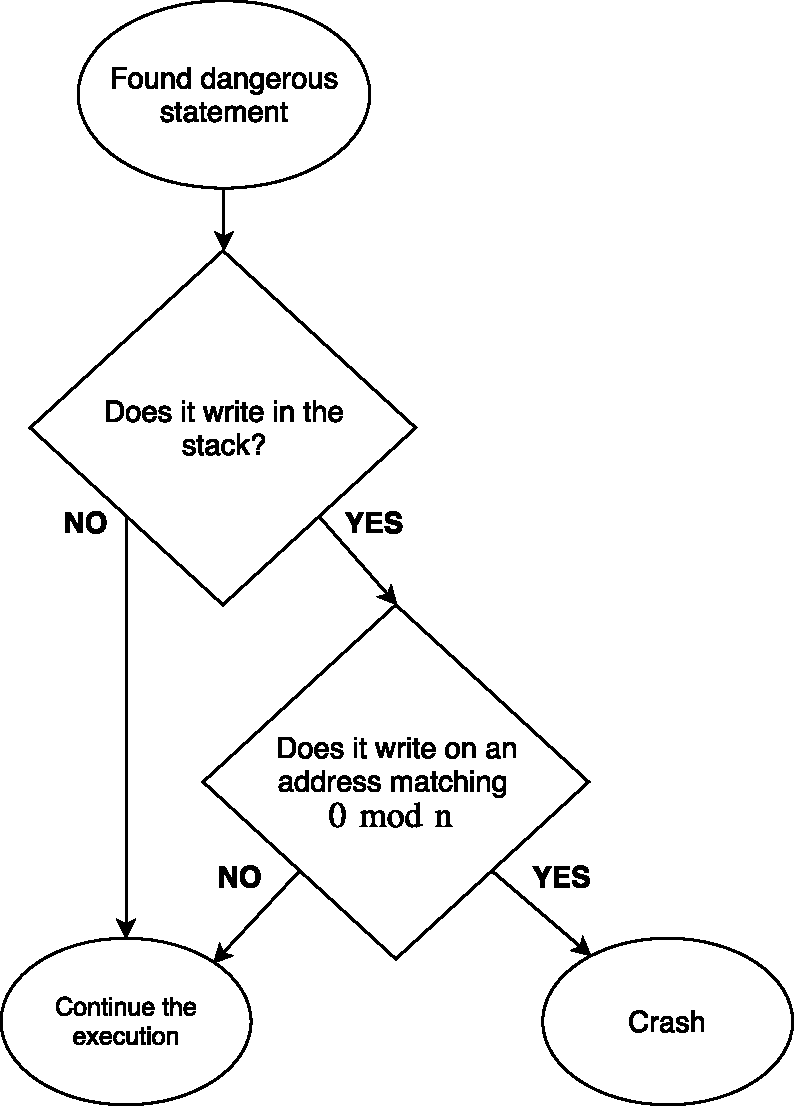
\includegraphics[scale=0.6]{images/runtime_check.pdf}
\caption{Runtime check algorithm}
\label{runtime_check}
\end{figure}

	To sum it up, our approach aims to have an easy way to know return addresses location and then add a check at runtime before every dangerous instruction to prevent illegal writing on return addresses location.
To do this we divided the approach into four phases:
\begin{enumerate}
	\item Fix stack frames size
	\item Align the stack
	\item Detect dangerous statements
	\item Secure the dangerous statements
\end{enumerate}


\subsection{Security properties}
\label{sub:Security properties}
	The approach we propose is composed of four phases, to get the confidence that our idea is effective in protecting return addresses we are going to formalize the properties we expect from each phase. 
Furthermore like we pointed earlier, we're going to work with the certified compiler CompCert.
The ideal way to be sure of our idea would be to prove it with Coq the proof assistant the language used to build CompCert.
By working with these tools we hope that one day we will be able to prove some security guarantees brought by our approach.

\begin{enumerate}
	\item \textbf{Fixed stack frames size}
		\begin{itemize}
			\item Return addresses locations are all separated by a constant offset equals to the size of the frames
			\item The transformation does not change the semantic of the module 
		\end{itemize}
	\item \textbf{Stack alignment}
		\begin{itemize}
			\item The first return address location of the stack have its least significant bits equals to 0
			\item The transformation does not change the semantic of the module 
		\end{itemize}
	\item \textbf{Detection of memory write statements}
		\begin{itemize}
			\item Every statement of the analysed code that might modify the stack memory state is detected
		\end{itemize}
	\item \textbf{Securing memory write statements}
		\begin{itemize}
			\item Statements that does not involve the protected addresses will keep their behaviour
			\item The protection will trigger an error behaviour if we try to write on a protected address
		\end{itemize}
\end{enumerate}

1. and 2. combined give us the guarantee that the least significant bits of all the return addresses location will be equal to $\mathbf{0~mod~n} \text{ with } n \text{ the size of the frames }$.

\hfill \break 
We make it so the protection mechanism prevents any write on addresses located in the \textbf{stack memory area} and their least significant bits equal to $\mathbf{0~mod~n}$.

\hfill \break 
If all these properties are fulfilled we are confident that under certain conditions it's not possible for a hazardous module to modify the flow control through the return addresses.
The necessary conditions for our approach to work will be discussed right after.

\subsection{Analysis of the approach}
\label{sub:Analysis of the approach}


\subsubsection{Conditions}
\label{ssub:Conditions}

We believe that the solution we've just presented can bring very strong security properties against ROP attacks. However for this approach to work we need certain hypothesis to be true. Indeed some of the properties enumerated before become false after certain operations.

\begin{itemize}
	\item \textbf{Stack modifications}, every operation that disrupts the stack structure may nullify our property that says ''every return addresses are separated by a fixed offset''. For example x86 architecture use the ESP register to keep track of the stack growth. If we fiddle with it we may introduce a shift in the return addresses location. Then our runtime check on $\mathbf{0~mod~n}$ addresses would not be relevant anymore.
		An example of such operation in C is inline assembly which allows us to put some assembly code in C code (Figure \ref{inline_assembly}). One simple solution to this flaw would be to forbid any usage of inline assembly.

	\item \textbf{Unsecure libraries}, for our approach to work we need to have all dangerous write statements to contain our runtime checks. Hence all executed code must have been compiled with our transformation. For example, the \textit{glibc} library of C contains multiple insecure functions like \textit{printf, strcpy\dots} Furthermore those flawed functions are common vulnerabilities for \textit{buffer overflows} attacks which are a type of ROP attack. To avoid this issue we would need to rewrite the glibc or compile it with our tools.
\end{itemize}

\begin{figure}
\begin{lstlisting}
int foo(int a) {
	asm(''sub 50, esp'');
	%asm(''sub $50, %esp'');
	//This line does the operation ESP = ESP - 50
	//This disrupts the stack layout we establish in our transformation
	printf("Hello world!");
}
\end{lstlisting}
\centering
\caption{C inline assembly}
\label{inline_assembly}
\end{figure}


Those conditions are necessary for our approach to be relevant. Yet we can't guarantee that these conditions are an exhaustive list of the hypothesis needed. They're the conditions we could think of but there might are some more.

\subsubsection{Discussion}
\label{ssub:Discussion}
	We have presented the principle of our approach in this chapter. Following we mentioned some necessary conditions for our solution to be relevant. In this section we're going to discuss about the pros, cons or remarks about the proposed solution.

	The benefits of our transformation is clear, any code compiled with a compiler enforcing our methods is unable to interfere with the control flow of our program through return addresses.
	Furthermore if we combine our solution with the SFI presented earlier we can have some strong security properties on the execution of dangerous modules with our main program.
Alas there are also some disadvantages to our approach that we're going to present here:
	\begin{itemize}
		\item \textbf{Architecture dependant}, our solution depends a lot of the stack layout of the program. Indeed fixing the size of the frames requires us to modify the original stack layout. Therefore since the stack layout vary depending of the architecture and compiler you're using, the modifications that have to be done are also different. We can then easily comprehend that we would need a different implementations for every existing stack layout. Moreover since these layouts can be really different it might be very gruesome to implement our solution on certain of them.
In the implementation we present after we focus solely on x86-32 architecture with the compiler CompCert.
		\item \textbf{Memory consumption}, since we're fixing the size of the frames instead of having dynamic sizes the memory usage of the stack is bigger. We have the issue of choosing an adequate size for the frames in our solution. The easiest one is to take the maximum frame size of the program as the constant size for all the frames. The downside is that we might have a memory usage explosion from our stack. To put a cost on the impact of our solution on the stack size we would need to make numerous tests. Unfortunately during the span of the internship we were unable to do so but it's one of our objectives for the remaining time.
	\end{itemize}

Despite the cons presented we believe the benefits we gain from this method is worth it. With regard to the negative impacts on stack memory consumption we personally didn't encounter any issue with the different tests we made our implementation go through. The impacts may be visible on especially big programs which we did not test yet.
We're going to present in the following section the implementation we made based on the ideas we introduced here. This implementation was made with the compiler CompCert for the x86-32 architecture. We're targeting programs written in C, which explains that all the examples we used were related to the C language.


\label{sec:section name}

\section{Implementation}
\label{sec:Implementation and analysis}

For the implementation of our idea we chose to work with the compiler CompCert. CompCert already had an implementation of SFI presented earlier. Thus if we could combine our approach with the SFI, any program compiled with CompCert would have strong security guarantees. Furthermore CompCert is written with Coq the proof assistant, we eventually hope that we will be able to prove these security properties. In this section we're going explain in details how we implemented the approach and the different choices we did during the process. Afterwards we will discuss these choices and evaluate the results and performance obtained.

\subsection{Implementation}
\label{sub:Implementation}
	Our approach is separated in four phases: ``Fixed stack frames size'', ``Stack alignment'', ``Detection of memory write statements'' and ``Evaluation of the implementation''. We're going detail the implementation of these phases in the following sections. These transformations are deeply linked to the stack layout, hence to have a better understanding we're going to start by introducing the CompCert stack structure.

\subsubsection{CompCert stack}
\label{ssub:CompCert stack}
	The layout of the stack is dependent of the architecture and the compiler/interpreter used. For a better understanding of the future sections we describe here the stack layout of x86-32 in CompCert.
First of all in x86 the stack grows downwards, it means that the stack grows from the highest addresses to the low ones.
A lot of information are saved in the stack, we can find the parameters of the functions, local variables, saved state of registers and the return address of the function.
In CompCert the stack layout is composed as in Figure \ref{stack_layout}.

\begin{figure}
\centering
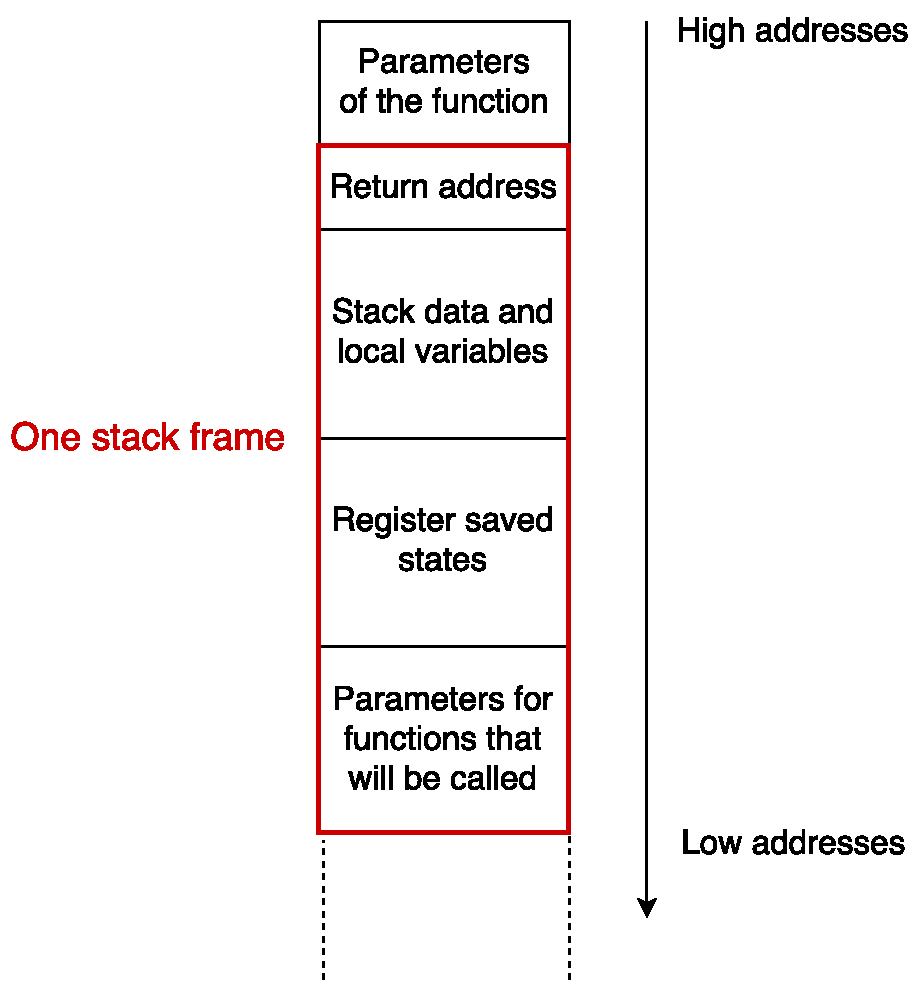
\includegraphics[scale=0.5]{images/stack_layout.pdf}
\caption{CompCert x86-32 stack layout}
\label{stack_layout}
\end{figure}

Each frame is built when a function is called, the different steps related to the creation of a frame is called \textit{function call routine}.
CompCert function call routine is described here and in the Figure \ref{call_routine}:
\begin{enumerate}
	\item Write the return address
	\item Allocate enough memory for the rest of the stack
	\item Save registers states in the stack
	\item Execute the function body (use the memory for local and stack data)
	\item When calling another function, place its parameters at the end of the stack and repeat the process
\end{enumerate}

\begin{figure}
\centering
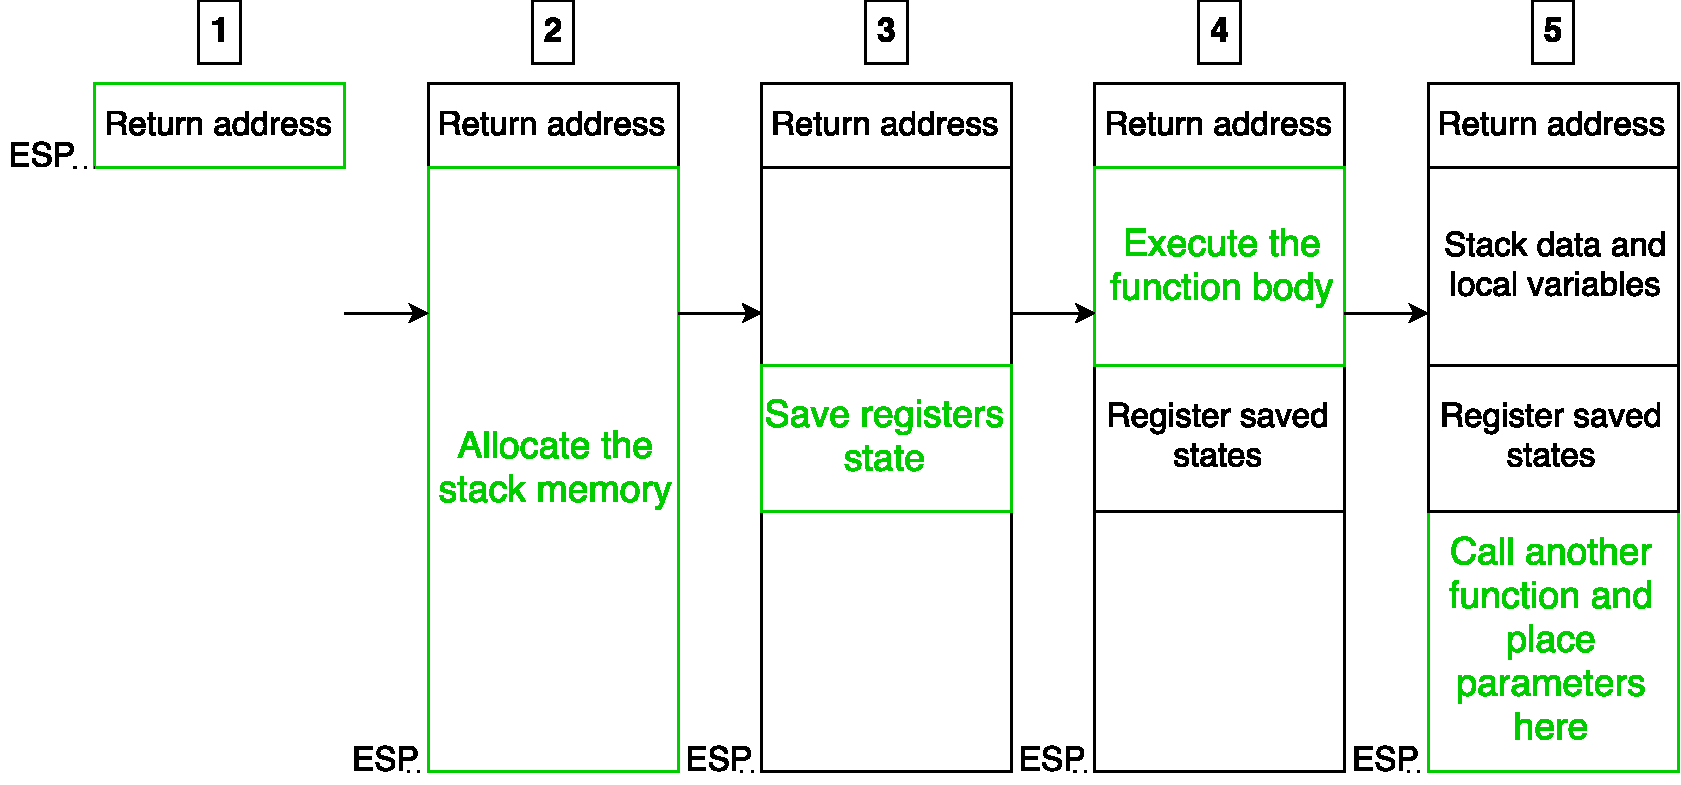
\includegraphics[scale=0.5]{images/call_routine.pdf}
\caption{CompCert function call routine}
\label{call_routine}
\end{figure}


When returning from a function it's pretty much the opposite:
\begin{enumerate}
	\item Restore registers state
	\item Deallocate the stack until the return addresses
	\item Pop the return address memory and jump to the value stored in it
\end{enumerate}




\subsubsection{Fixed stack frames size}
\label{sub:Fixed stack frames size}

\subsubsection{Stack alignment}
\label{ssub:Stack alignment}

\subsubsection{Detection of memory write statements}
\label{ssub:Detection of memory write statements}

\subsubsection{Securing memory write statements}
\label{ssub:Securing memory write statements}

\subsection{Evaluation of the implementation}
\label{sub:Evaluation of the implementation}





\end{document}
%%% Local Variables:
%%% mode: latex
%%% TeX-master:
%%% End:

